\title{Pevné Látky}
\documentclass[10pt,a4paper]{article}
\usepackage[utf8]{inputenc}
\usepackage[czech]{babel}
\usepackage{amsmath}
\usepackage{amsfonts}
\usepackage{amssymb}
\usepackage{chemfig}
\usepackage{geometry}
\usepackage{wrapfig}
\usepackage{graphicx}
\usepackage{floatflt}
\usepackage{hyperref}
\usepackage{fancyhdr}
\usepackage{tabularx}
\usepackage{makecell}
\usepackage{csquotes}
\usepackage{footnote}
\usepackage{movie15}
\MakeOuterQuote{"}

\renewcommand{\labelitemii}{$\circ$}
\renewcommand{\labelitemiii}{--}
\newcommand{\ra}{$\rightarrow$ }
\newcommand{\x}{$\times$ }
\newcommand{\lp}[2]{#1 -- #2}
\newcommand{\timeline}{\input{timeline}}


\geometry{lmargin = 0.8in, rmargin = 0.8in, tmargin = 0.8in, bmargin = 0.8in}
\date{\today}
\author{Jakub Rádl}

\makeatletter
\let\thetitle\@title
\let\theauthor\@author
\makeatother

\hypersetup{
colorlinks=true,
linkcolor=black,
urlcolor=cyan,
}



\begin{document}
\maketitle
\tableofcontents
\begin{figure}[b]
Toto dílo \textit{\thetitle} podléhá licenci Creative Commons \href{https://creativecommons.org/licenses/by-nc/4.0/}{CC BY-NC 4.0}.\\ (creativecommons.org/licenses/by-nc/4.0/)
\end{figure}
\newpage


\section{Pevné látky}
\begin{enumerate}
\item Jaká je nejpevnější látka? (tvrdost -- diamant, tah -- pavoučí vlákna, dnes uhlíková nanovlákna, \ldots)
\item Jaká jsou využití křemíku? (polovodiče, silikony, \ldots)
\item Proč mají sněhové vločky pravidelný tvar? (díky úhlům v molekule $H_2O$ tvoří 6-úhelník, krystalizuje okolo krystalizačních jader)
\item Co je to koeficient bezpečnosti? (udává, kolikrát více produkt vydrží oproti tomu, na kolik je hodnocen)
\item Co je to nanotechnologie? (technologie $<$ 100nm např. počítačové čipy)
\end{enumerate}

\section{Struktura pevných látek}
\subsection{Atomy a chemické vazby}
\paragraph{Vazby}
\begin{itemize}
\item \textbf{kovalentní} (nevodiče)
\item \textbf{kovová} (umožňuje volný pohyb elektronů -> vodiče)
\item \textbf{iontová} 
\item slabé (vodíková, \ldots)
\end{itemize}

\paragraph{Rozdělení látek}
\begin{itemize}
\item \textbf{monokrystalické} -- pravidelná struktura (diamant, křemík)
\item \textbf{polykrystalické} -- pravidelná struktura v rozdělených oblastech na mikroskopické úrovni (kovy, led)
\item \textbf{amorfní} -- absolutně nepravidelná struktura (sklo, vosk, makromolekulární látky)
\end{itemize}
Mezi amorfními a polykrystalickými látkami je těžko rozlišitelná hranice.
\begin{itemize}
\item \textbf{směsi} (beton)
\end{itemize}


\subsection{Vlastnosti monokrystalů}
\begin{itemize}
\item \textbf{pravidelnost}
\item \textbf{kmitání atomů} kolem rovnovážných poloh
\end{itemize}

\paragraph{Krystalová mřížka}
\begin{itemize}
\item určuje geometrickou souměrnost
\item 7 soustav (matematicky dokázáno, že jich nemůže být více)
\begin{itemize}
	\item krychlová, jednoklonná, trojklonná, klencová, šesterečná, čtverečná, kosočtverečná
\end{itemize}
\end{itemize}

\paragraph{Elementární buňka}
\begin{itemize}
\item základní jednotka krystalu, periodicky se opakuje
\end{itemize}

\paragraph{Př.: železo $\alpha$}\mbox{}\\ \mbox{} \\
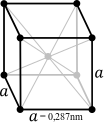
\includegraphics[scale=0.5]{pictures/001.png}
\footnote{https://upload.wikimedia.org/wikipedia/commons/a/a3/Cubic-body-centered.svg}
\begin{itemize}
\item elementární buňkou jsou pouze vnitřní jeden rohový atom
\end{itemize}

\paragraph{Př.: spočítejte hustotu železa z informací o jeho el. buňce}
\begin{itemize}
\item $\rho = \frac{m}{V} = \frac{2 \cdot m_{Fe} }{a^3} = \frac{2 \cdot A_r \cdot m_u }{a^3} = \frac{2 \cdot 56 \cdot 1.66 \cdot 10^{-27}}{(0.287 \cdot 10^{-9})^3} \doteq 7864kg \cdot m^{-3} $
\end{itemize}
pozn.: Struktura a velikost krystalu se určuje pomocí rentgenové difrakce. 

\paragraph{Př.: struktura diamantu}\mbox{}\\ \mbox{} \\
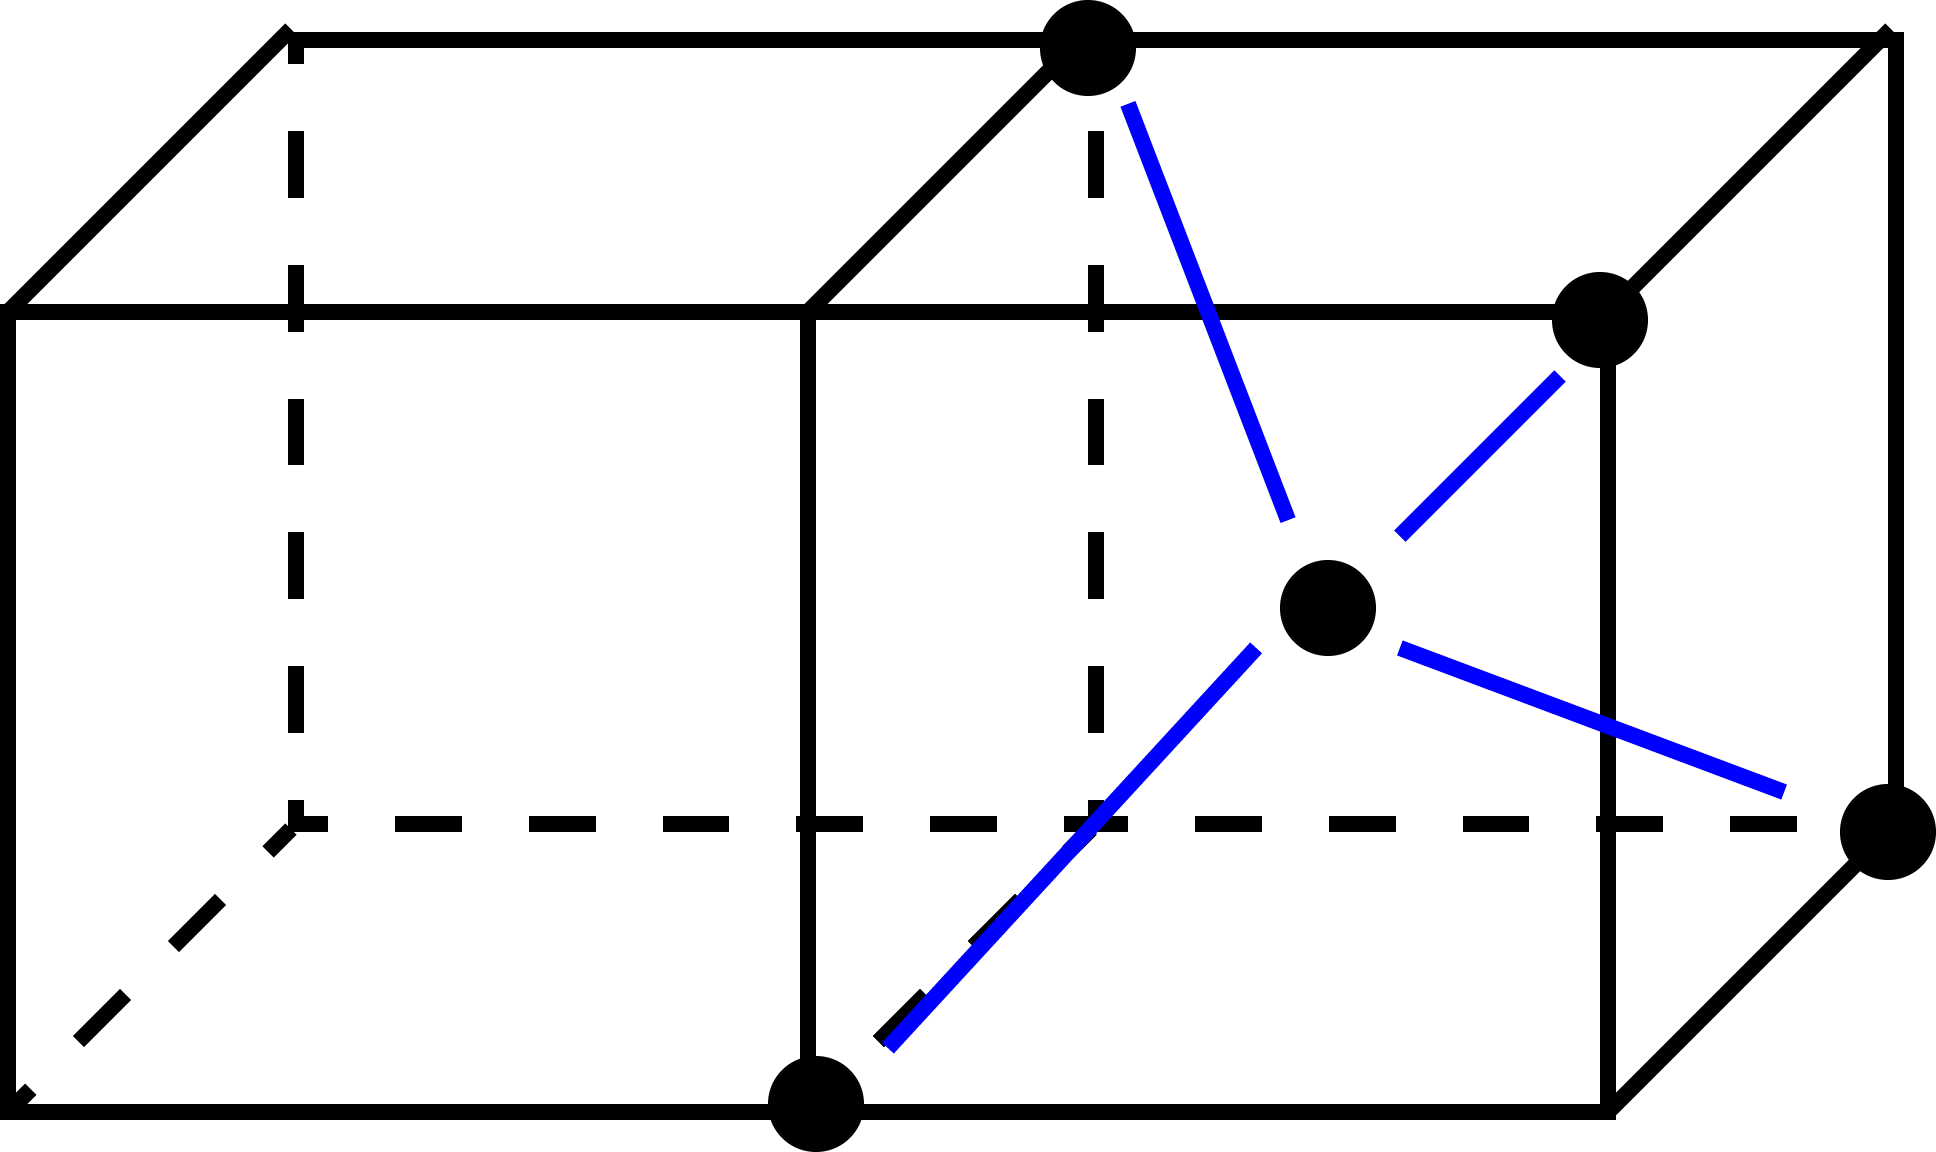
\includegraphics[width=0.25\textwidth]{pictures/002.png}

\paragraph{Př.: struktura fullerenu}\mbox{}\\ \mbox{} \\
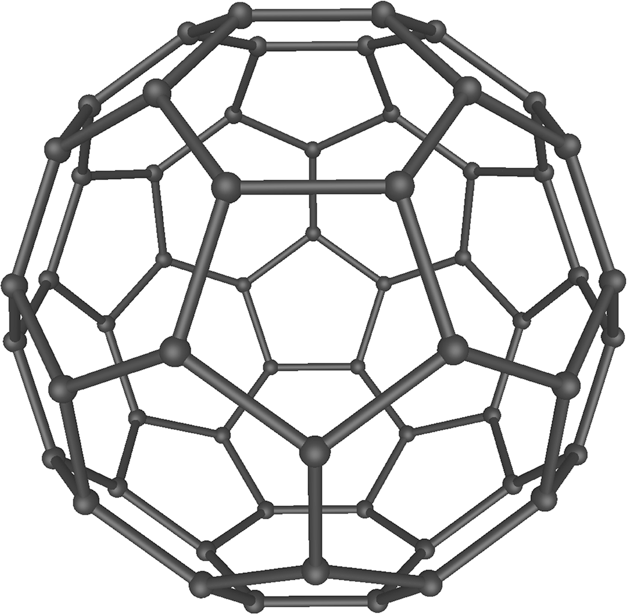
\includegraphics[width=0.25\textwidth]{pictures/003.png}
\footnote{https://upload.wikimedia.org/wikipedia/commons/4/41/C60a.png}

\paragraph{Př.: struktura grafitu}\mbox{}\\ \mbox{} \\
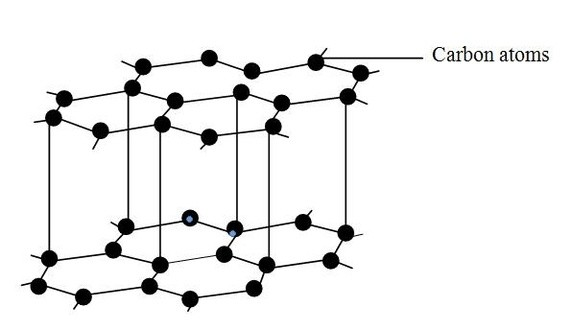
\includegraphics[width=0.4\textwidth]{pictures/004.jpg}
\footnote{https://i.stack.imgur.com/dqwRb.jpg}


\paragraph{Reálný krystal}
\begin{enumerate}
\item obsahuje příměsi $\rightarrow$ změna vlastností
\item poruchy pravidelnosti
\begin{itemize}
\item dislokace
\end{itemize}
\end{enumerate}

\end{document}